\subsubsection{PCB Hardware Elements}

The hardware subsystem forms the foundation of the drone, integrating all power, control, and sensing elements on a custom PCB. It is designed to be compact, lightweight, and serviceable while maintaining electrical reliability, EMI resilience, and thermal performance. Figure~\ref{fig:pcb-sections} illustrates the overall hardware and firmware architecture.

\begin{figure}[H]
    \centering
    \captionsetup{justification=centering, margin=1cm}
    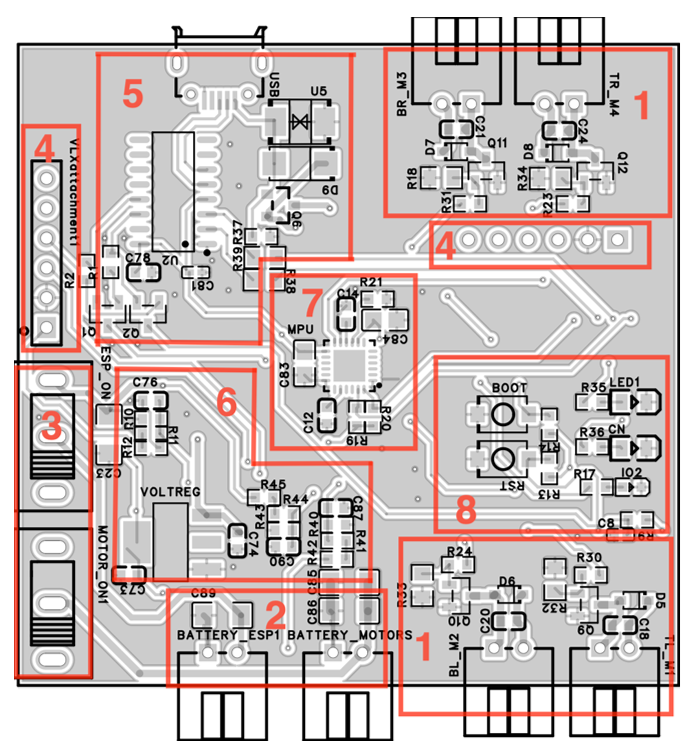
\includegraphics[width=0.5\textwidth]{img/pcb-sections2.PNG}
    \caption{Areas of PCB design}
    \label{fig:pcb-sections}
\end{figure}

\begin{table}[h!]
\centering
\caption{Hardware Element Legend}
\label{tab:hardware-legend}
\begin{tabular}{|c|l|}
\hline
\rowcolor{gray!15}\textbf{No.} & \textbf{Hardware Element} \\ \hline
1 & Motor Drivers \\ \hline
2 & Battery Terminals \\ \hline
3 & Switch \\ \hline
4 & Distance Sensor Attachments \\ \hline
5 & UART Communication \\ \hline
6 & Voltage Regulation \\ \hline
7 & Motion Tracking \\ \hline
8 & Boot/Reset Buttons \& Safety LEDs \\ \hline
\end{tabular}
\end{table}

The intent and the description of various hardware elements is given Table~\ref{tab:hardware-elements}.

\pagebreak

\begin{longtable}{@{}p{2cm} p{6.9cm} p{6.9cm}@{}}
\caption{Summary of Hardware Elements and Their Design Intent}
\label{tab:hardware-elements} \\
\toprule
\textbf{Element} & \textbf{Intent \& Requirements} & \textbf{Design Description} \\ 
\midrule
\textbf{Motor Drivers} &
\textit{Intent:} Drive brushed motors safely with low EMI and adequate thermal margin. \newline
\textit{Requirements:} R.23 low cost; A.R.6 case temperature $\leq 85~^{\circ}$C; supply droop $\leq 10\%$ at full duty; EMI interference-free I\textsuperscript{2}C communication. &
Motor drivers are placed near PCB edges to minimise path resistance and EMI. Flyback diodes and RC snubbers reduce transients; short, wide power returns and local decoupling capacitors enhance current stability. \\ 
\midrule
\textbf{Battery Terminals} &
\textit{Intent:} Provide a robust and safe connection for 1S/2S Li-ion/LiPo power. \newline
\textit{Requirements:} R.18/A.R.2 single-battery operation; reverse insertion blocked; voltage drop $\leq 100$~mV at max current. &
Locking JST-style connector with keyed housing ensures polarity. Bulk capacitors stabilize voltage input; wide copper pours minimise resistance to LDO and driver rails. \\ 
\midrule
\textbf{Power Switch (Enable)} &
\textit{Intent:} Allow user-controlled power activation without arcing or brownout. \newline
\textit{Requirements:} R.17 safety handling; voltage sag $\leq 5\%$ on 3.3~V rail. &
RC debounce implemented; switch positioned away from propellers with silkscreen labels and visual LED indicators for power status. \\ 
\midrule
\textbf{Distance Sensor Attachments} &
\textit{Intent:} Enable obstacle avoidance and altitude hold. \newline
\textit{Requirements:} R.11/R.12 obstacle sensing; I\textsuperscript{2}C error rate = 0 during PWM activity. &
Two 4-pin headers (GND/VCC/SCL/SDA) with onboard pull-ups for optional sensor modules; mechanical mounting aligns with forward and downward sensing directions. \\ 
\midrule
\textbf{UART/USB Communication} &
\textit{Intent:} Support flashing and telemetry without disassembly. \newline
\textit{Requirements:} AF.R.9 flashing success $\geq 99\%$; A.R.10 accessible during assembly; ESD robustness. &
CP2102/CH340 bridge with ESD protection and reverse-current Schottky diode on 5~V. Connector side-mounted for tool-free firmware updates. \\ 
\midrule
\textbf{Voltage Regulation (3.3~V Rail)} &
\textit{Intent:} Provide stable, low-noise 3.3~V power for MCU and IMU. \newline
\textit{Requirements:} Output within $\pm5\%$; regulator temp $\leq 85~^{\circ}$C under full load. &
Linear LDO provides noise-free supply; distributed decoupling and thermal copper pours dissipate heat efficiently. \\ 
\midrule
\textbf{Motion Tracking (IMU)} &
\textit{Intent:} Deliver accurate attitude measurement with minimal vibration coupling. \newline
\textit{Requirements:} R.20 stabilisation; placement within $\pm3$~mm of centroid; reliable I\textsuperscript{2}C/SPI interface. &
IMU placed centrally for balanced dynamics; shielded traces and ground guards minimise noise; isolated from high-current return paths. \\ 
\midrule
\textbf{Boot/Reset Buttons \& Safety LEDs} &
\textit{Intent:} Provide clear feedback and safe recovery during operation. \newline
\textit{Requirements:} A.R.7/A.R.10 indicators visible at 0.5~m; accessible with props installed. &
BOOT/EN buttons near board edge for easy reach; tri-state LEDs communicate idle, connected, and low-battery states; spacing ensures no RF interference. \\ 
\bottomrule
\end{longtable}

%-------------------------------------------------------------%
\subsubsection{Frame Design Elements}

The frame provides mechanical protection, airflow, and structural support while accommodating sensors, cameras, and cabling. Each component was designed for serviceability, modularity, and weight efficiency while preserving the drone’s balance and stability.

\begin{longtable}{@{}p{3.2cm} p{6.4cm} p{6.4cm}@{}}
\toprule
\textbf{Element} & \textbf{Intent \& Requirements} & \textbf{Design Description} \\ 
\midrule

\textbf{Camera Mount (Front Facing)} &
\textit{Intent:} Maintain clear FOV and low vibration for stable imaging. \newline
\textit{Requirements:} R.28/R.29 video; R.2/R.20 stability; quick-swap $\leq 60$~s. &
Snap-on carrier with compliant flexure arms isolates vibration; unobstructed optical path; easily replaceable. \\ 
\midrule

\textbf{Antenna \& LED Keep-Outs} &
\textit{Intent:} Ensure RF integrity and LED visibility. \newline
\textit{Requirements:} A.R.7/A.R.10 indicators visible at 0.5~m; antenna free of obstruction. &
Keep-out zones near ESP32 antenna edge maintained; LEDs exposed through open frame for visibility and heat dissipation. \\ 
\midrule

\textbf{Cable Management \& Strain Relief} &
\textit{Intent:} Prevent interference with propellers and ensure safe wiring. \newline
\textit{Requirements:} A.R.6 mechanical safety; cable retention $\geq$ 15~N. &
Dedicated tie-points and routing along arms; cables secured away from rotors and heat zones. \\ 
\midrule

\textbf{Serviceability \& Replacement} &
\textit{Intent:} Enable rapid repair and part replacement. \newline
\textit{Requirements:} Replaceable parts; print time $\leq$ 3~h for any component. &
Tool-less snap-fit assembly with modular arms and carriers; low-cost reprinting workflow. \\ 
\midrule

\textbf{Crash Protection \& Mass Control} &
\textit{Intent:} Absorb impact energy and protect electronics. \newline
\textit{Requirements:} R.23 cost/weight; prevent critical damage in collisions. &
Sacrificial PETG prop guards and legs designed to fail first, shielding PCB and motors during impact. \\ 
\bottomrule
\end{longtable}

\begin{figure}[H]
    \centering
    \captionsetup{justification=centering, margin=1cm}
    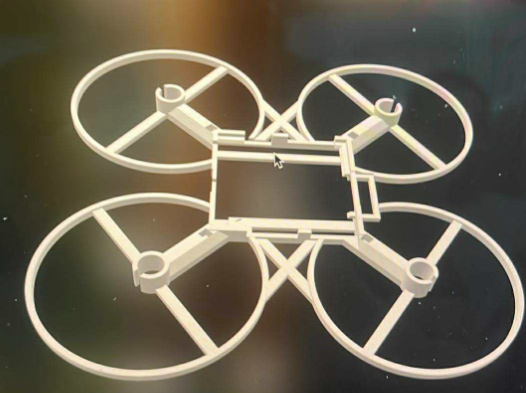
\includegraphics[width=0.5\textwidth]{img/frame-placeholder.PNG}
    \caption{Frame design \temp{Placeholder image}}
    \label{fig:pcb-sections}
\end{figure}
